
Language technologies are information technologies specialised in human
language processing. Therefore these technologies are also often
subsumed under the term human language technology. Human language occurs
in spoken and written form. While speech is the oldest and most natural
mode of language communication, complex information and the bulk of
human knowledge is recorded and transmitted in written texts. Speech and
text technologies process or produce language in these two forms.
However, language also has aspects common to both forms such as
dictionaries, most of the grammar, and the meaning of sentences. Thus,
large parts of language technology cannot be subsumed under either
speech or text technologies. Knowledge technologies include technologies
that link language to knowledge. Figure \ref{fig:ltincontexten} illustrates the language
technology in context. In our communication, we mix language with other
modes of communication and other information media. We combine speech
with gestures and facial expressions. Texts can be combined with
pictures and sounds. Films may contain language in spoken and written
form. Thus, speech and text technologies overlap and interact with many
other technologies that facilitate the processing of multi-modal
communication and multimedia documents.

\begin{figure*}[htb]
  \colorrule{grey3}{\textwidth}{1.5pt}
  \center
  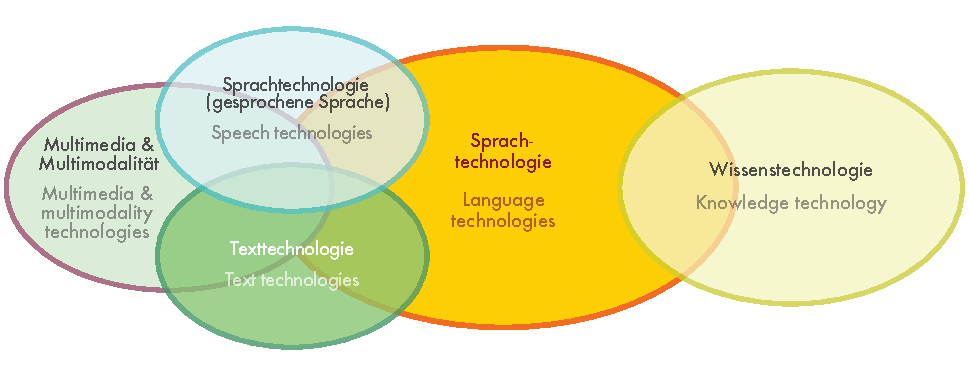
\includegraphics[width=\textwidth]{../_media/english/language_technologies}
  \caption{Language technology in context}
  \label{fig:ltincontexten}
  \colorrule{grey3}{\textwidth}{1.5pt}
\end{figure*}

